% =============================================================================
%  slides_nishioka.tex  ─  Conference Presentation
%  "GPU-Accelerated Bayesian Inference of Multi-Species Biofilm
%   Interaction Parameters via TMCMC"
%  K. Nishioka, F. Klempt, H. Geisler, M. Soleimani, P. Junker
%  IKM, Leibniz Universität Hannover  ·  2026
% =============================================================================
\documentclass[aspectratio=169,10pt,t]{beamer}

% ── Packages ─────────────────────────────────────────────────────────────────
\usepackage[utf8]{inputenc}
\usepackage[T1]{fontenc}
\usepackage{lmodern}
\usepackage{microtype}
\usepackage{amsmath,amssymb,bm}
\usepackage{booktabs,array,multirow}
\usepackage{graphicx}
\usepackage{tikz}
\usetikzlibrary{arrows.meta,positioning,shapes.geometric,backgrounds,decorations.pathreplacing,calc}
\usepackage{xcolor}
\usepackage{caption,subcaption}
\usepackage{appendixnumberbeamer}   % restarts frame counter in appendix
\usepackage{colortbl}
\usepackage{ragged2e}
\usepackage[numbers,sort&compress]{natbib}

\graphicspath{%
  {figures/}%
  {paper_figures/}%
  {../FEM/figures/paper_final/}%
  {../data_5species/experiment_fig/}%
  {../data_5species/docs/paper_comprehensive_figs/}%
}

% ── Colour palette ───────────────────────────────────────────────────────────
\definecolor{ikm}      {RGB}{0,82,147}
\definecolor{ikmdark}  {RGB}{0,55,100}
\definecolor{ikmlight} {RGB}{224,237,249}
\definecolor{ikmxlight}{RGB}{240,247,255}
\definecolor{red2}     {RGB}{200,40,30}
\definecolor{green2}   {RGB}{20,140,60}
\definecolor{gold}     {RGB}{195,145,0}
\definecolor{lightgray2}{RGB}{245,245,248}
\definecolor{midgray}  {RGB}{110,110,110}

% ── Base theme ───────────────────────────────────────────────────────────────
\usetheme{default}
\usecolortheme{default}
\usefonttheme[onlymath]{serif}
\setbeamertemplate{navigation symbols}{}
\setbeamertemplate{blocks}[rounded][shadow=false]
\setbeamersize{text margin left=0.45cm, text margin right=0.45cm}

% ── Colors ───────────────────────────────────────────────────────────────────
\setbeamercolor{frametitle}         {bg=ikm,         fg=white}
\setbeamercolor{title}              {fg=ikm}
\setbeamercolor{subtitle}           {fg=ikmdark}
\setbeamercolor{block title}        {bg=ikm,         fg=white}
\setbeamercolor{block body}         {bg=ikmxlight}
\setbeamercolor{alertblock title}   {bg=red2,        fg=white}
\setbeamercolor{alertblock body}    {bg=red2!8}
\setbeamercolor{exampleblock title} {bg=green2,      fg=white}
\setbeamercolor{exampleblock body}  {bg=green2!8}
\setbeamercolor{structure}          {fg=ikm}
\setbeamercolor{item}               {fg=ikm}
\setbeamercolor{subitem}            {fg=ikmdark}
\setbeamercolor{section in toc}     {fg=ikm}
\setbeamercolor{background canvas}  {bg=white}

% ── Fonts ────────────────────────────────────────────────────────────────────
\setbeamerfont{title}         {size=\LARGE,  series=\bfseries,  family=\sffamily}
\setbeamerfont{subtitle}      {size=\large,  series=\mdseries,  family=\sffamily}
\setbeamerfont{author}        {size=\small,                      family=\sffamily}
\setbeamerfont{institute}     {size=\small,                      family=\sffamily}
\setbeamerfont{date}          {size=\small,                      family=\sffamily}
\setbeamerfont{frametitle}    {size=\normalsize, series=\bfseries, family=\sffamily}
\setbeamerfont{block title}   {size=\small,  series=\bfseries,  family=\sffamily}
\setbeamerfont{block body}    {size=\footnotesize,               family=\sffamily}
\setbeamerfont{section in toc}{size=\small,  series=\bfseries}

% ── Frametitle: icon + text in one blue bar ───────────────────────────────────
\setbeamertemplate{frametitle}{%
  \nointerlineskip
  \begin{beamercolorbox}[wd=\paperwidth,ht=0.60cm,dp=0.20cm,leftskip=0.45cm]{frametitle}%
    \usebeamerfont{frametitle}\insertframetitle%
  \end{beamercolorbox}%
}

% ── Footline ─────────────────────────────────────────────────────────────────
\setbeamertemplate{footline}{%
  \leavevmode%
  \hbox{%
    \begin{beamercolorbox}[wd=.55\paperwidth,ht=2.0ex,dp=1ex,leftskip=4pt]{structure}%
      \usebeamerfont{footline}\color{midgray}\tiny\insertshortauthor
      \ifx\insertsectionhead\empty\else\quad\textbullet\quad\insertsectionhead\fi
    \end{beamercolorbox}%
    \begin{beamercolorbox}[wd=.45\paperwidth,ht=2.0ex,dp=1ex,rightskip=6pt,right]{structure}%
      \usebeamerfont{footline}\color{midgray}\tiny
      \insertframenumber\,/\,\inserttotalframenumber
    \end{beamercolorbox}}%
  \vskip0pt%
}

% (No automatic section divider slides)

% ── List spacing ─────────────────────────────────────────────────────────────
\setlength{\leftmargini}{1.3em}
\setlength{\leftmarginii}{1.1em}
\setbeamertemplate{itemize item}  {\small\raisebox{0.12ex}{\color{ikm}$\blacktriangleright$}}
\setbeamertemplate{itemize subitem}{\scriptsize\raisebox{0.12ex}{\color{ikmdark}--}}
\setbeamertemplate{enumerate item}{\small\textbf{\color{ikm}\insertenumlabel.}}

% ── Caption style ────────────────────────────────────────────────────────────
\captionsetup{font=scriptsize,labelfont={color=ikm,bf},skip=1pt}

% ── Macros ───────────────────────────────────────────────────────────────────
\newcommand{\btheta}{\boldsymbol{\theta}}
\newcommand{\bphi}{\boldsymbol{\phi}}
\newcommand{\bpsi}{\boldsymbol{\psi}}
\newcommand{\bphibar}{\bar{\boldsymbol{\phi}}}
\newcommand{\yobs}{\mathbf{y}_{\mathrm{obs}}}
\newcommand{\hl}[1]{\textbf{\textcolor{ikm}{#1}}}
\newcommand{\hlr}[1]{\textbf{\textcolor{red2}{#1}}}
\newcommand{\hlg}[1]{\textbf{\textcolor{green2}{#1}}}
\newcommand{\citeref}[1]{{\tiny[\cite{#1}]}}

% ── Title ─────────────────────────────────────────────────────────────────────
\title[GPU-Bayes Biofilm TMCMC]{%
  GPU-Accelerated Bayesian Inference\\
  of Multi-Species Biofilm Interaction Parameters\\
  via TMCMC}
\subtitle{Full Discovery of 15-Dimensional Interaction Matrix}
\author[Nishioka et al.]{%
  \textbf{Keisuke Nishioka}$^{1}$,\;
  Felix Klempt$^{1}$,\;
  Hendrik Geisler$^{1}$,\;
  Meisam Soleimani$^{1}$,\;
  Philipp Junker$^{1}$\\[3pt]
  Nils Heine$^{2}$,\;
  Kristina Bittroff$^{2}$,\;
  Szymon P.\ Szafranski$^{2}$,\;
  Meike Stiesch$^{2}$}
\institute[IKM/NIFE]{%
  $^1$Institute of Continuum Mechanics, Leibniz Universit\"at Hannover\\
  $^2$NIFE, Medizinische Hochschule Hannover}
\date{2026}

% =============================================================================
\begin{document}
% =============================================================================

% ── Title slide ───────────────────────────────────────────────────────────────
\begin{frame}[plain]
  \begin{tikzpicture}[remember picture,overlay]
    \fill[ikm]     (current page.north west) rectangle ([yshift=-0.11\paperheight]current page.north east);
    \fill[ikmlight](current page.south west) rectangle ([yshift= 0.18\paperheight]current page.south east);
    \fill[ikm]     (current page.south west) rectangle ([yshift= 0.045\paperheight]current page.south east);
  \end{tikzpicture}
  \vspace{0.6cm}
  \begin{center}
    {\sffamily\bfseries\large\color{ikm}
      GPU-Accelerated Bayesian Inference of\\[4pt]
      Multi-Species Biofilm Interaction Parameters via TMCMC\par}
    \vspace{0.30cm}
    {\color{ikm!60!black}\rule{0.65\textwidth}{0.6pt}\par}
    \vspace{0.22cm}
    {\sffamily\small\color{ikmdark}
      Full Discovery of the 15-Dimensional Interaction Matrix
      with Two-Phase GPU-TMCMC\par}
    \vspace{0.55cm}
    {\sffamily\small
      \textbf{Keisuke Nishioka}$^1$,\ Felix Klempt$^1$,\ Hendrik Geisler$^1$,\
      Meisam Soleimani$^1$,\ Philipp Junker$^1$\par}
    \vspace{4pt}
    {\sffamily\footnotesize
      Nils Heine$^2$,\ Kristina Bittroff$^2$,\ Szymon P.\ Szafranski$^2$,\
      Meike Stiesch$^2$\par}
    \vspace{4pt}
    {\sffamily\footnotesize\color{midgray}
      $^1$IKM, Leibniz Universit\"at Hannover\quad
      $^2$NIFE, MHH Hannover\par}
    \vspace{0.45cm}
    {\sffamily\footnotesize\color{midgray} 2026}
  \end{center}
\end{frame}

% ── Outline ───────────────────────────────────────────────────────────────────
\begin{frame}{Outline}
  \tableofcontents[hideallsubsections]
\end{frame}

% =============================================================================
\section{Motivation \& Background}
% =============================================================================

\begin{frame}[t]{Peri-Implantitis and Multi-Species Biofilm Dysbiosis}
  \small\vspace{-2pt}
  \begin{columns}[T]
    \column{0.54\textwidth}
      \begin{block}{Clinical problem}
        \begin{itemize}\setlength{\itemsep}{2pt}
          \item \hl{Peri-implantitis}: inflammatory bone destruction around dental implants
          \item Primary driver: multi-species oral biofilm \textbf{dysbiosis}
            \cite{Marsh2003Dental}
          \item Prevalence $\sim$20\% of implant patients \cite{EarlyImplantBiofilm2024}
          \item Structural mechanics of the biofilm change with community state
        \end{itemize}
      \end{block}
      \vspace{4pt}
      \begin{block}{Open question}
        \begin{itemize}\setlength{\itemsep}{2pt}
          \item \textbf{Which} inter-species interactions drive the commensal$\to$dysbiotic transition?
          \item \textbf{How stiff} does the biofilm become, and what stresses does it exert?
          \item Current gap: no quantitative, data-driven parameter estimation framework
        \end{itemize}
      \end{block}
      \vspace{4pt}
      \textbf{This work:} Bayesian inference of \hl{15 interaction parameters} from in-vitro time-series data, validated against 4 conditions
    \column{0.44\textwidth}
      \vspace{4pt}
      \centering
      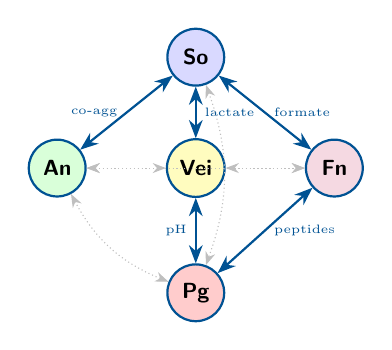
\begin{tikzpicture}[scale=0.88, every node/.style={transform shape},
          sp/.style={circle,draw=ikm,thick,minimum size=0.82cm,font=\small\bfseries\sffamily},
          confirmed/.style={<->,thick,>=Stealth,ikm},
          unknown/.style={<->,thin,gray!50,>=Stealth,densely dotted}
      ]
        \node[sp,fill=blue!15]   (so)  at (0,   2.3) {So};
        \node[sp,fill=green!15]  (an)  at (-2.0, 0.7) {An};
        \node[sp,fill=yellow!25] (vei) at (0,   0.7) {Vei};
        \node[sp,fill=purple!15] (fn)  at (2.0, 0.7) {Fn};
        \node[sp,fill=red!20]    (pg)  at (0,  -1.1) {Pg};
        \draw[confirmed] (so)--(an)  node[midway,left,font=\tiny]  {co-agg};
        \draw[confirmed] (so)--(vei) node[midway,right,font=\tiny] {lactate};
        \draw[confirmed] (so)--(fn)  node[midway,right,font=\tiny] {formate};
        \draw[confirmed] (vei)--(pg) node[midway,left,font=\tiny]  {pH};
        \draw[confirmed] (fn)--(pg)  node[midway,right,font=\tiny] {peptides};
        \draw[unknown]   (an)--(vei);
        \draw[unknown]   (an)--(fn);
        \draw[unknown]   (vei)--(fn);
        \draw[unknown]   (so) to[bend left=20]  (pg);
        \draw[unknown]   (an) to[bend right=20] (pg);
      \end{tikzpicture}
      \vspace{3pt}
      {\scriptsize
       \textcolor{ikm}{$\longleftrightarrow$} Confirmed pathway\quad
       \textcolor{gray}{$\cdots$} Free parameter\par}
      \vspace{4pt}
      {\scriptsize Indexing: So=1, An=2, Vei=3, Fn=4, Pg=5}
  \end{columns}
\end{frame}

\begin{frame}[t]{Heine et al.\ (2025): Four-Condition Time-Series Dataset}
  \small\vspace{-2pt}
  \begin{columns}[T]
    \column{0.50\textwidth}
      \begin{block}{Experimental design \cite{Heine2025PeriImplant}}
        \begin{itemize}\setlength{\itemsep}{2pt}
          \item 5 oral species: So, An, Vei, Fn, Pg
          \item \textbf{4 conditions}: Commensal $\times$ \{Static, HOBIC\},
                Dysbiotic $\times$ \{Static, HOBIC\}
          \item \textbf{6 time points}: Days 1, 3, 6, 10, 15, 21
          \item $N=8$ biological replicates per condition
          \item HOBIC = biofilm reactor mimicking gingival fluid flow
        \end{itemize}
      \end{block}
      \vspace{4pt}
      \begin{block}{Key distinction: Pg strain}
        \begin{itemize}\setlength{\itemsep}{2pt}
          \item \textbf{Commensal}: Pg ATCC\,20709 (avirulent, non-encapsulated)
          \item \textbf{Dysbiotic}: Pg W83 (virulent, complete gingipain \& fimbrial genes)
        \end{itemize}
      \end{block}
      \vspace{4pt}
      Data normalised to volume fractions $\phi_i \in [0,1]$;\;
      Day 1 = initial condition, $N_t=5$ usable time points per species
    \column{0.48\textwidth}
      \vspace{2pt}
      \centering
      \includegraphics[width=\linewidth,height=0.58\textheight,keepaspectratio]%
        {expected_heatmap.png}
      \par\vspace{2pt}
      {\scriptsize Heatmap: mean $\langle\phi_i(t_k)\rangle_{N=8}$ across conditions.
       Dysbiotic conditions show late Pg surge (Day 15--21).}
  \end{columns}
\end{frame}

% =============================================================================
\section{5-Species Interaction Network}
% =============================================================================

\begin{frame}[t]{Five Key Oral Species and Their Confirmed Interactions}
  \small\vspace{-2pt}
  \begin{columns}[T]
    \column{0.42\textwidth}
      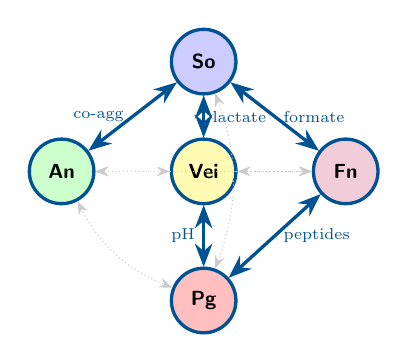
\begin{tikzpicture}[scale=0.82, every node/.style={transform shape},
          sp/.style={circle,draw=ikm,very thick,minimum size=1.0cm,font=\small\bfseries\sffamily},
          confirmed/.style={<->,very thick,>=Stealth,ikm},
          unknown/.style={<->,thin,gray!40,>=Stealth,densely dotted}
      ]
        \node[sp,fill=blue!20]   (so)  at (0,   2.5) {So};
        \node[sp,fill=green!20]  (an)  at (-2.2, 0.8) {An};
        \node[sp,fill=yellow!30] (vei) at (0,   0.8) {Vei};
        \node[sp,fill=purple!20] (fn)  at (2.2, 0.8) {Fn};
        \node[sp,fill=red!25]    (pg)  at (0,  -1.2) {Pg};
        \draw[confirmed] (so)--(an)  node[midway,left,font=\scriptsize]  {co-agg};
        \draw[confirmed] (so)--(vei) node[midway,right,font=\scriptsize] {lactate};
        \draw[confirmed] (so)--(fn)  node[midway,right,font=\scriptsize] {formate};
        \draw[confirmed] (vei)--(pg) node[midway,left,font=\scriptsize]  {pH};
        \draw[confirmed] (fn)--(pg)  node[midway,right,font=\scriptsize] {peptides};
        \draw[unknown]   (an)--(vei); \draw[unknown] (an)--(fn);
        \draw[unknown]   (vei)--(fn);
        \draw[unknown]   (so) to[bend left=20]  (pg);
        \draw[unknown]   (an) to[bend right=20] (pg);
      \end{tikzpicture}
    \column{0.56\textwidth}
      \renewcommand{\arraystretch}{1.15}
      \begin{tabular}{@{}p{1.3cm}p{3.2cm}p{2.1cm}@{}}
        \toprule
        \textbf{Pair} & \textbf{Mechanism} & \textbf{Ref.}\\
        \midrule
        So--An & Co-aggregation; So provides growth substrates for An
          & \cite{Kolenbrander2010OralMultispecies}\\
        So--Vei & Lactate production by So; Vei consumes lactate to elevate pH
          & \cite{Kolenbrander2010OralMultispecies}\\
        So--Fn & Formate symbiosis; Fn bridges early--late colonisers
          & \cite{Kolenbrander2010OralMultispecies}\\
        Vei$\to$Pg & Vei creates alkaline micro-niche favourable to Pg (pH $\uparrow$)
          & \cite{Heine2025PeriImplant}\\
        Fn--Pg & Fn provides peptide nutrients; physical co-aggregation with Pg
          & \cite{Kolenbrander2010OralMultispecies}\\
        \bottomrule
      \end{tabular}
      \vspace{5pt}
      \begin{block}{Pg virulence: W83 strain}
        \begin{itemize}\setlength{\itemsep}{1pt}
          \item Gingipains (Arg/Lys-specific proteases): tissue degradation
          \item Fimbriae: adhesion and invasion of epithelial cells
          \item Lipopolysaccharide: immunoevasion \cite{Mukherjee2025PgTitanium}
          \item Absent in commensal ATCC\,20709
        \end{itemize}
      \end{block}
      \vspace{4pt}
      {\scriptsize\color{midgray}
       Dotted grey: no confirmed pathway; all 15 parameters estimated freely.}
  \end{columns}
\end{frame}

% =============================================================================
\section{Mathematical Framework}
% =============================================================================

\begin{frame}[t]{Continuum Biofilm Model: State Variables}
  \small\vspace{-2pt}
  \begin{columns}[T]
    \column{0.48\textwidth}
      \begin{block}{State variables (per material point)}
        \begin{itemize}\setlength{\itemsep}{2pt}
          \item $\phi_i \in [0,1]$: volume fraction of species $i$
          \item $\psi_i \in [0,1]$: viability fraction (membrane-intact cells)
          \item $\bar\phi_i := \phi_i\psi_i$: \emph{living} volume fraction
          \item $\phi_0$: void / fluid phase
          \item $\gamma(t)$: Lagrange multiplier
        \end{itemize}
      \end{block}
      \vspace{6pt}
      \textbf{Volume constraint}:
      \[
        \sum_{l=0}^{5}\phi_l(t) = 1 \quad\forall\,t
      \]
      \vspace{4pt}
      \begin{alertblock}{Key modelling choice}
        $\bar\phi_i = \phi_i\psi_i$: growth is driven by \emph{living} cells,
        not total biomass\\
        $\Rightarrow$ captures cell death independently of volume change
      \end{alertblock}
    \column{0.50\textwidth}
      \begin{block}{Extended Hamilton Principle \cite{JunkerBalzani2021ExtendedHamilton}}
        \[
          \mathcal{H} = \int_\tau \bigl(\underbrace{\mathcal{G}}_{\text{free energy}}
                        + \underbrace{\mathcal{C}}_{\text{constraint}}
                        + \underbrace{\mathcal{D}}_{\text{dissipation}}\bigr)\,\mathrm{d}t
          \;\to\; \mathrm{stat}_{\boldsymbol{\xi},\gamma}
        \]
      \end{block}
      \vspace{6pt}
      \textbf{Free energy} (nutrient-driven growth, $\alpha^*\!=0$):
      \[
        \Psi = -\tfrac{1}{2}\,c^*\,\bphibar^{\top}\!\mathbf{A}\,\bphibar
      \]
      \textbf{Dissipation potential}:
      \[
        \mathcal{D}
        = \tfrac{1}{2}\dot{\bphibar}^{\top}\!\boldsymbol{\eta}\,\dot{\bphibar}
        + \tfrac{1}{2}\dot{\bphi}^{\top}\!\boldsymbol{\eta}\,\dot{\bphi}
      \]
      \[
        \boldsymbol{\eta}=\mathrm{diag}(\eta_i),\quad \eta_i=1\quad\text{(normalised)}
      \]
      \vspace{4pt}
      {\scriptsize\color{midgray}
       Barrier $\Psi_\mathrm{bar}=K_p/[\phi_i^2(1-\phi_i)^2]$
       enforces $\phi_i,\psi_i\in(0,1)$ numerically.}
  \end{columns}
\end{frame}

\begin{frame}[t]{Symmetric Interaction Matrix: 15 Free Parameters}
  \small\vspace{-2pt}
  \begin{columns}[T]
    \column{0.52\textwidth}
      \begin{block}{Symmetric interaction matrix $\mathbf{A}$}
        \[
          \mathbf{A}\in\mathbb{R}^{5\times5},\quad A_{ij}=A_{ji}
          \;\Rightarrow\; \btheta=\{a_{ij}\}_{i\le j}\;\in\mathbb{R}^{15}
        \]
        \[
          \mathbf{A}=\begin{pmatrix}
            a_{11} & a_{12} & a_{13} & a_{14} & a_{15}\\
                   & a_{22} & a_{23} & a_{24} & a_{25}\\
                   &        & a_{33} & a_{34} & a_{35}\\
                   &        &        & a_{44} & a_{45}\\
                   &        &        &        & a_{55}
          \end{pmatrix}
        \]
        \vspace{2pt}
        $A_{ij}>0$: mutualism/cross-feeding\quad
        $A_{ij}<0$: competition\\
        $A_{ii}>0$: self-facilitated growth (density dependence)
      \end{block}
    \column{0.46\textwidth}
      \vspace{4pt}
      \begin{block}{Full-discovery approach}
        \begin{itemize}\setlength{\itemsep}{3pt}
          \item All 15 parameters estimated \emph{without a priori locking}
          \item Biological sparsity (Pg$\approx0$ in commensal)
                emerges from the posterior
          \item Symmetry $A_{ij}=A_{ji}$ enforced by variational structure
        \end{itemize}
      \end{block}
      \vspace{6pt}
      \begin{exampleblock}{Governing ODE (from $\delta\mathcal{H}=0$)}
        \[
          0 = -c^*\psi_i\bigl(\mathbf{A}\bphibar\bigr)_i
              + \eta_i\bigl(\dot\phi_i\psi_i^2+\bar\phi_i\dot\psi_i+\dot\phi_i\bigr)
              + \gamma
        \]
        \[
          0 = -c^*\phi_i\bigl(\mathbf{A}\bphibar\bigr)_i
              + \eta_i\bigl(\dot\psi_i\phi_i^2+\bar\phi_i\dot\phi_i\bigr)
              + \gamma
        \]
      \end{exampleblock}
      \vspace{3pt}
      {\scriptsize\color{midgray}
       $c^*=25$, $\eta_i=1$, $\Delta t=10^{-4}$, $N_t^{\mathrm{sim}}=2500$ steps}
  \end{columns}
\end{frame}

% =============================================================================
\section{Bayesian Inference via TMCMC}
% =============================================================================

\begin{frame}[t]{Bayesian Framework: Likelihood and Prior}
  \small\vspace{-2pt}
  \begin{columns}[T]
    \column{0.50\textwidth}
      \textbf{Posterior} \cite{RobertCasella2004MonteCarlo}:
      \[
        p(\btheta\mid\yobs)
        \propto \underbrace{p(\yobs\mid\btheta)}_{\text{likelihood}}\,
                \underbrace{p(\btheta)}_{\text{prior}}
      \]
      \vspace{2pt}
      \begin{block}{Gaussian likelihood}
        \[
          \ln p(\yobs\mid\btheta)
          = -\sum_{k,i}\frac{(y_{i,k}-\hat y_{i,k}(\btheta))^2}{2\sigma_i^2}
        \]
        $\sigma_i$: species-specific replicate s.d.\\
        ($\approx0.05$ for Fn/Pg commensal; $\approx0.20$ for So)\\[2pt]
        $N=8$ biological replicates per condition
      \end{block}
      \vspace{4pt}
      \begin{block}{Constrained uniform prior}
        \[
          p(\btheta)=\prod_{k=0}^{14}\frac{1}{u_k-l_k}\,\mathbf{1}_{[l_k,u_k]}(\theta_k)
        \]
        Bounds iteratively narrowed after Phase 1:\\
        $[q_{0.01}-1.5\sigma,\;q_{0.99}+1.5\sigma]$
      \end{block}
    \column{0.48\textwidth}
      \vspace{4pt}
      \begin{block}{Identifiability challenge}
        \begin{itemize}\setlength{\itemsep}{2pt}
          \item $N_t=5$ usable time points $\times$ 5 species $=$ 25 observations
          \item 15 unknowns $\Rightarrow$ near-saturation of information content
          \item Coupled $\phi_i$--$\psi_i$ dynamics: multimodal posterior landscape
          \item Standard MCMC: inefficient / stuck in local modes
        \end{itemize}
      \end{block}
      \vspace{6pt}
      \begin{alertblock}{Our solution: TMCMC + two-phase strategy}
        \begin{enumerate}\setlength{\itemsep}{2pt}
          \item \textbf{Phase 1}: fix $\psi_i$, halve ODE dim, remove $\psi$-modes
          \item \textbf{TMCMC}: tempered likelihood for global exploration
          \item \textbf{GPU}: $N_p=10{,}000$ particles feasible in $\sim$2\,h
        \end{enumerate}
      \end{alertblock}
      \vspace{4pt}
      By-product: log model evidence $\ln\hat Z$\,\;
      (used for Bayes factor model selection)
  \end{columns}
\end{frame}

\begin{frame}[t]{Two-Phase Estimation Strategy}
  \small
  \vspace{4pt}
  \begin{center}
  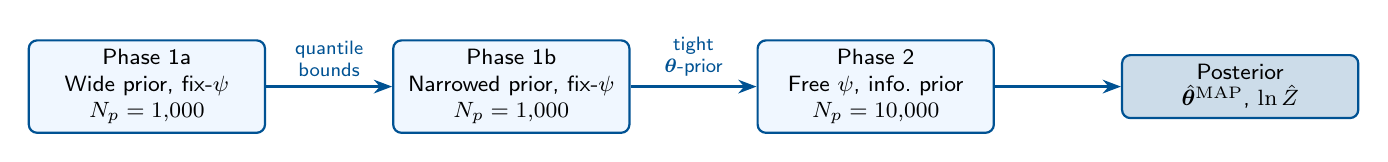
\begin{tikzpicture}[
    node distance=0.6cm and 1.6cm,
    box/.style={rectangle,rounded corners=3pt,draw=ikm,thick,fill=ikmxlight,
                minimum width=3.0cm,minimum height=0.78cm,align=center,
                font=\sffamily\footnotesize},
    arrow/.style={->,thick,>=Stealth,ikm},
    label/.style={font=\sffamily\scriptsize\color{midgray},align=center}
  ]
    \node[box]              (p1a) {Phase 1a\\Wide prior, fix-$\psi$\\$N_p=1{,}000$};
    \node[box,right=of p1a] (p1b) {Phase 1b\\Narrowed prior, fix-$\psi$\\$N_p=1{,}000$};
    \node[box,right=of p1b] (p2)  {Phase 2\\Free $\psi$, info.\ prior\\$N_p=10{,}000$};
    \node[box,right=of p2,fill=ikm!20] (out) {Posterior\\$\hat\btheta^{\mathrm{MAP}}$, $\ln\hat Z$};
    \draw[arrow] (p1a) -- node[above,label]{quantile\\bounds} (p1b);
    \draw[arrow] (p1b) -- node[above,label]{tight\\$\btheta$-prior} (p2);
    \draw[arrow] (p2)  -- (out);
  \end{tikzpicture}
  \end{center}
  \vspace{4pt}
  \begin{columns}[T]
    \column{0.49\textwidth}
      \begin{block}{Phase 1: fix-$\psi$ mode (robust)}
        \begin{itemize}\setlength{\itemsep}{2pt}
          \item Set $\psi_i(t_k) \leftarrow \psi_i^{\mathrm{exp}}(t_k)$ (measured)
          \item Eliminates viability-related posterior modes
          \item Halves ODE Jacobian dimension
          \item Provides tight $\btheta$-bounds for Phase 2
        \end{itemize}
      \end{block}
    \column{0.49\textwidth}
      \begin{block}{Phase 2: free-$\psi$ mode (joint posterior)}
        \begin{itemize}\setlength{\itemsep}{2pt}
          \item Release $\psi_i$ as free variables
          \item Viability as \emph{soft} constraint:
                $\ln\mathcal{L}\,{+}{=}\,-\sum(\psi_i-\psi_i^{\exp})^2/(2\cdot0.1^2)$
          \item Phase 1 posterior $\Rightarrow$ informative $\btheta$-prior
          \item Physically consistent joint $(\mathbf{A},\bpsi)$ posterior
        \end{itemize}
      \end{block}
  \end{columns}
\end{frame}

% =============================================================================
\section{GPU-Accelerated Implementation}
% =============================================================================

\begin{frame}[t]{JAX + vmap on GPU: \hl{$\sim$200$\times$} Speedup}
  \small\vspace{-2pt}
  \begin{columns}[T]
    \column{0.52\textwidth}
      \begin{block}{Computational challenge}
        $\mathcal{O}(10^5\text{--}10^6)$ ODE solves per TMCMC run\\
        ($N_p=10{,}000$ particles $\times$ 20 MH steps $\times$ $\sim$5 stages)
      \end{block}
      \vspace{5pt}
      \textbf{JAX implementation} \cite{Bradbury2018JAX}:
      \begin{itemize}\setlength{\itemsep}{2pt}
        \item Implicit Euler--Newton solver: \texttt{jax.jit} compiled
        \item Entire particle ensemble: \texttt{jax.vmap} on GPU
        \item Single fused XLA kernel — zero Python overhead per solve
        \item RW-TMCMC avoids variable-length leapfrog
          (NUTS/HMC: GPU warp divergence)
      \end{itemize}
      \vspace{5pt}
      \begin{block}{Adaptive $\gamma$-scaling}
        Init: $\gamma^2=2.38^2/15$ (Roberts--Rosenthal optimal for $d=15$)\\
        Online: halve if $\bar\alpha<5\%$;\enspace
        $\times1.5$ if $\bar\alpha>40\%$
      \end{block}
    \column{0.46\textwidth}
      \centering\vspace{4pt}
      \renewcommand{\arraystretch}{1.12}
      \begin{tabular}{@{}lrrr@{}}
        \toprule
        \textbf{Metric} & \textbf{CPU} & \textbf{GPU} & \textbf{Speedup}\\
        \midrule
        \multicolumn{4}{@{}l}{\textit{Matched benchmark ($N_p=500$, DH):}}\\
        \quad Per stage   & 2{,}400\,s & 14\,s   & $170\times$\\
        \quad Total       & 21{,}600\,s & 147\,s & \hl{$\mathbf{200\times}$}\\
        \midrule
        \multicolumn{4}{@{}l}{\textit{Production ($N_p=10{,}000$):}}\\
        \quad Per cond.  & $\sim$120\,h$^\dagger$ & 1.7--2.6\,h & $\sim$50$\times$\\
        \quad 4 cond.    & $\sim$480\,h$^\dagger$ & 8\,h & $\sim$60$\times$\\
        \bottomrule
      \end{tabular}
      \vspace{4pt}
      {\scriptsize $^\dagger$Extrapolated from 500-particle CPU benchmark}
      \vspace{8pt}

      \textbf{Hardware}: NVIDIA RTX\,4090 (24\,GB VRAM)\\
      \textbf{CPU baseline}: 12-core Intel Xeon\\[6pt]
      \hlr{$\sim$200$\times$ speedup} (matched settings)\\
      Production $N_p=10{,}000$ feasible in $\sim$\hl{2\,h}/condition
    \end{columns}
\end{frame}

% =============================================================================
\section{Results}
% =============================================================================

\begin{frame}[plain]{Posterior Predictive Fits: All 4 Conditions}
  \vspace{-2pt}
  \centering
  
\includegraphics[height=0.84\textheight,keepaspectratio]{paper_fig2_phi_transposed.png}
  \par\vspace{2pt}
  {\color{midgray}\rule{0.88\textwidth}{0.3pt}}\par\vspace{1pt}
  {\scriptsize
   Columns: CS, CH, DS, DH (increasing dysbiotic severity)\enspace
   Rows: So, An, Vei, Fn, Pg\enspace
   Solid line: MAP $\phi_i$\enspace
   Dashed: living fraction $\bar\phi_i$\enspace
   Shaded: 50\%/80\% CI (100 posterior samples)}
\end{frame}

\begin{frame}[plain]{Inferred Interaction Matrices: Commensal vs.\ Dysbiotic}
  \vspace{-2pt}
  \centering
  
\includegraphics[height=0.76\textheight,keepaspectratio]{heatmap_A_4cond.png}
  \par\vspace{2pt}
  {\color{midgray}\rule{0.88\textwidth}{0.3pt}}\par
  \begin{columns}[T]
    \column{0.5\textwidth}
      {\scriptsize\textbf{Commensal (CS, CH):} So--An and So--Vei blocks dominant;\enspace
       Fn, Pg entries $\approx0$ (emergent sparsity without locking)}
    \column{0.5\textwidth}
      {\scriptsize\textbf{Dysbiotic (DS, DH):} Strong Vei$\to$Pg (pH) + Fn$\to$Pg (peptides);\enspace
       $\hat a_{45}^{\mathrm{DH}}=5.63$\enspace (Fn--Pg); $\hat a_{55}^{\mathrm{DH}}=3.43$}
  \end{columns}
\end{frame}

\begin{frame}[plain]{Posterior Parameter Distributions (Phase 2, $N_p=10{,}000$)}
  \vspace{-2pt}
  \centering
  
\includegraphics[height=0.82\textheight,keepaspectratio]{paper_posterior_violin.pdf}
  \par\vspace{2pt}
  {\color{midgray}\rule{0.88\textwidth}{0.3pt}}\par\vspace{1pt}
  {\scriptsize
   All 15 $\mathbf{A}$-entries.\enspace
   Stars: MAP.\enspace
   CS/CH: Pg-related params ($a_{15},a_{25},a_{35},a_{45},a_{55}$) concentrate near zero
   \emph{without a priori locking}.\enspace
   DS: narrowest posteriors (best identifiability).}
\end{frame}

\begin{frame}[t]{Quantitative Fit Metrics and Phase Consistency}
  \small\vspace{4pt}
  \begin{columns}[T]
    \column{0.52\textwidth}
      \centering
      \renewcommand{\arraystretch}{1.25}
      \begin{tabular}{@{}l rr rr r@{}}
        \toprule
        & \multicolumn{2}{c}{\textbf{Phase 1}} & \multicolumn{2}{c}{\textbf{Phase 2 (final)}}
        & \\
        \cmidrule(lr){2-3}\cmidrule(lr){4-5}
        \textbf{Cond.} & RMSE & MAE & RMSE & MAE & $\ln\hat Z$\\
        \midrule
        CS & 0.119 & 0.077 & 0.119 & 0.075 & $-3.3$\\
        CH & 0.071 & 0.053 & 0.104 & 0.088 & $-8.5$\\
        DS & \hl{\textbf{0.020}} & \hl{\textbf{0.025}} & \hl{\textbf{0.033}} & \hl{\textbf{0.024}} & $\mathbf{-2.8}$\\
        DH & 0.067 & 0.045 & 0.087 & 0.060 & $-11.9$\\
        \bottomrule
      \end{tabular}
      \vspace{6pt}
      {\scriptsize Phase 1: fix-$\psi$,\; $N_p=1{,}000$\quad
       Phase 2: free $\psi$,\; $N_p=10{,}000$}
      \vspace{10pt}

      \begin{block}{Phase MAP consistency ($r$ = Pearson)}
        \begin{itemize}\setlength{\itemsep}{3pt}
          \item CS: $r=0.87$ (fix-$\psi$ already valid)
          \item CH: $r=0.68$ (acceptable)
          \item DS: $r=0.42$ (Phase 2 essential)
          \item DH: $r=0.62$ (shift in $a_{55},a_{45}$)
        \end{itemize}
      \end{block}
    \column{0.46\textwidth}
      \begin{block}{Observations}
        \begin{itemize}\setlength{\itemsep}{4pt}
          \item DS: lowest RMSE $=$ \hl{0.033} (best identifiability)
          \item Phase 2 $\Delta$RMSE $\leq0.03$: Phase\,1 robust
          \item DH Pg: gingipain $r=\hlg{0.90}$ (independent)
        \end{itemize}
      \end{block}
      \vspace{8pt}
      \begin{block}{TMCMC Convergence}
        \begin{itemize}\setlength{\itemsep}{4pt}
          \item $M=4$--7 tempering stages
          \item Acceptance rate $\bar\alpha=7$--13\%
          \item ESS $=N_p$ at final stage
          \item Gelman--Rubin $\hat R<1.1$ (all params)
        \end{itemize}
      \end{block}
  \end{columns}
\end{frame}

\begin{frame}[t]{Cross-Condition Transferability and Independent Validation}
  \small\vspace{-2pt}
  \begin{columns}[T]
    \column{0.46\textwidth}
      \textbf{Cross-condition transfer RMSE}
      \vspace{3pt}
      \renewcommand{\arraystretch}{1.1}
      \begin{tabular}{@{}lccccc@{}}
        \toprule
        & \multicolumn{4}{c}{\textbf{Target}} \\
        \cmidrule{2-5}
        \textbf{Source} & CS & CH & DS & DH \\
        \midrule
        CS & \textit{.273} & \hl{\textbf{.135}} & \hl{\textbf{.111}} & .244 \\
        CH & .229 & \textit{.168} & \hl{\textbf{.127}} & .233 \\
        DS & .273 & .130 & \textit{.062} & .252 \\
        DH & .301 & .129 & \hlg{\textbf{.044}} & \textit{.262} \\
        \bottomrule
      \end{tabular}
      \vspace{2pt}
      {\scriptsize Italic: self-prediction.\quad Bold/colour: transfer $<$ self.}
      \vspace{4pt}
      \begin{alertblock}{Topological reorganisation}
        $\rho(\mathrm{DH}{-}\mathrm{CS})=-0.49$\\
        Health$\to$Disease $\neq$ parameter rescaling
      \end{alertblock}
    \column{0.52\textwidth}
      \textbf{Independent validation} (not used in fitting)
      \vspace{3pt}
      \begin{itemize}\setlength{\itemsep}{3pt}
        \item[\hlg{$\checkmark$}] \textbf{pH prediction}:
          $R^2=\hlg{0.71}$, $r=0.84$ ($N=12$ held-out)\\
          {\scriptsize $\mathrm{pH}=6.95-0.74\,\phi_{\mathrm{So}}-0.48\,\phi_{\mathrm{Vei}}$\;
           (lactate-driven acidification)}
        \item[\hlg{$\checkmark$}] \textbf{Gingipain--Pg correlation}:
          $r=\hlg{0.90}$ (5 time points, DH)\\
          {\scriptsize Both show delayed onset at Day 15--21}
        \item[\hlg{$\checkmark$}] \textbf{Metabolic sign consistency}:\\
          {\scriptsize MAP $A_{12}=+0.76$ (An$\to$Vei): lactate/succinate cross-feeding $\checkmark$}\\
          {\scriptsize MAP $A_{13}=-2.73$ (So$\to$Vei): niche competition dominates}
        \item[\hlg{$\checkmark$}] \textbf{Growth rate parity}:
          1.68\,h (comm.) $\approx$ 1.64\,h (dysb.)\\
          {\scriptsize Differences arise from interactions, not individual fitness}
      \end{itemize}
  \end{columns}
\end{frame}

% =============================================================================
\section{Multiscale FEM Extension}
% =============================================================================

\begin{frame}[plain]{End-to-End Differentiable Multiscale Pipeline}
  \vspace{-2pt}
  \centering
  
\includegraphics[height=0.86\textheight,keepaspectratio]{Fig20_e2e_pipeline.png}
  \par\vspace{2pt}
  {\color{midgray}\rule{0.88\textwidth}{0.3pt}}\par\vspace{1pt}
  {\scriptsize
   TMCMC posterior $\to$ MAP $\btheta$
   $\to$ Hamilton ODE $\to$ $\phi_i^{\mathrm{eq}}$
   $\to$ Dysbiosis Index (DI)
   $\to$ $E(\mathrm{DI})$
   $\to$ 3D FEM (Abaqus/JAX-FEM)}
\end{frame}

\begin{frame}[t]{Spatial DI Field and FEM Mechanical Results}
  \vspace{2pt}
  \begin{columns}[T]
    \column{0.50\textwidth}
      \centering
      
\includegraphics[width=\linewidth,height=0.52\textheight,keepaspectratio]{Fig10_di_field.png}\\[2pt]
      {\scriptsize\textbf{Dysbiosis Index $\mathrm{DI}(x,y)$} — 2D Hamilton+nutrient PDE.\\
       DH: $\mathrm{DI}\!\in\![0.22,0.89]$;\quad CS: $\mathrm{DI}\!\approx\!0.1$}
    \column{0.48\textwidth}
      \centering
      
\includegraphics[width=\linewidth,height=0.52\textheight,keepaspectratio]{Fig13_stress.png}\\[2pt]
      {\scriptsize\textbf{von Mises stress + displacement} — 3D conformal FEM\\
       17\,970 nodes, C3D4; GCF pressure $p_0=10$\,Pa}
  \end{columns}
  \vspace{6pt}
  \begin{columns}[T]
    \column{0.50\textwidth}
      \small
      \textbf{Stiffness}: CS \hl{$E\!\approx\!909$\,Pa} vs.\ DS \hlr{$E\!\approx\!32$\,Pa}\\
      \textbf{Ratio}: \hl{$28\times$ stiffness},\; \hl{$29.4\times$ displacement}
    \column{0.48\textwidth}
      \small
      $E(\mathrm{DI})=E_{\max}(1\!-\!\mathrm{DI})^n+E_{\min}\mathrm{DI}^n$,\; $n\!=\!2$\\
      {\scriptsize (rigidity percolation $f\!\approx\!2.0$;\; $E_{\max}\!=\!1000$\,Pa, $E_{\min}\!=\!10$\,Pa)}
  \end{columns}
\end{frame}

% =============================================================================
\section{Conclusions}
% =============================================================================

\begin{frame}[t]{Discussion: Biological Interpretation}
  \small\vspace{-2pt}
  \begin{columns}[T]
    \column{0.50\textwidth}
      \begin{block}{Commensal state (CS, CH)}
        \begin{itemize}\setlength{\itemsep}{2pt}
          \item So--An co-aggregation + So--Vei lactate exchange:\\
                \textbf{stable mutualistic core}
          \item Fn, Pg entries emerge near zero: data-driven sparsity
          \item HOBIC flow shifts So abundance but preserves community topology
          \item CS basin highly fragile: 49/51 perturbations jump to DI$\approx0.85$
        \end{itemize}
      \end{block}
      \vspace{5pt}
      \begin{block}{Dysbiotic transition mechanism}
        \begin{itemize}\setlength{\itemsep}{2pt}
          \item Vei$\to$Pg (pH) + Fn$\to$Pg (peptides) strongly activated by W83
          \item $\rho(\mathrm{DH}{-}\mathrm{CS})=-0.49$: \textbf{topological reorganisation}
          \item Not recoverable by parameter rescaling
          \item Within-state DH$\to$DS transfer RMSE = 0.044 (beats DS self 0.062)
        \end{itemize}
      \end{block}
    \column{0.48\textwidth}
      \begin{block}{Model parsimony (effective dimensionality)}
        Compression ratio: $r_i=\sigma_{\mathrm{post},i}/\Delta_{\mathrm{prior}}$
        ($\Delta_{\mathrm{prior}}=6$)\vspace{3pt}
        \begin{itemize}\setlength{\itemsep}{1pt}
          \item All 15 params: $r_i<0.43$ in every condition
          \item DS tightest: mean $r=0.07$ (very tight)
          \item Pg-related in commensal: $r_i\leq0.10$
          \item[$\Rightarrow$] Posterior shrinks them, not prior-dominated
        \end{itemize}
        \vspace{3pt}
        \hl{Full 15-parameter model justified.}
      \end{block}
      \vspace{5pt}
      \begin{exampleblock}{FEM connection}
        \begin{itemize}\setlength{\itemsep}{1pt}
          \item TMCMC $\btheta$ $\to$ DI field $\to$ $E(\mathrm{DI})$
          \item $28\times$ stiffness range: measurable mechanical signature of dysbiosis
          \item Posterior UQ propagated through entire pipeline
        \end{itemize}
      \end{exampleblock}
  \end{columns}
\end{frame}

\begin{frame}[t]{Conclusions}
  \small\vspace{-2pt}
  \begin{columns}[T]
    \column{0.49\textwidth}
      \begin{block}{1.\ Two-Phase Full-Discovery TMCMC}
        \begin{itemize}\setlength{\itemsep}{2pt}
          \item Phase 1 (fix-$\psi$): rapid, robust $\mathbf{A}$ identification
          \item Phase 2 (free $\psi$): joint posterior, physically consistent
          \item All \hl{15 parameters} free — emergent sparsity from data
        \end{itemize}
      \end{block}
      \vspace{4pt}
      \begin{block}{2.\ GPU-Accelerated TMCMC}
        \begin{itemize}\setlength{\itemsep}{2pt}
          \item JAX + \texttt{vmap} on RTX\,4090: \hl{$\sim$200$\times$ speedup}
          \item $N_p=10{,}000$ in \hl{$\sim$2\,h} per condition
          \item Production runs of 15D posteriors now feasible
        \end{itemize}
      \end{block}
    \column{0.49\textwidth}
      \begin{block}{3.\ Validated Biological Interpretation}
        \begin{itemize}\setlength{\itemsep}{2pt}
          \item pH: $r=\hlg{0.84}$;\quad Gingipain: $r=\hlg{0.90}$
          \item Commensal: So-centred mutualistic core
          \item Dysbiosis = topological reorganisation ($\rho=-0.49$)
        \end{itemize}
      \end{block}
      \vspace{4pt}
      \begin{block}{4.\ Multiscale FEM Extension}
        \begin{itemize}\setlength{\itemsep}{2pt}
          \item $28\times$ stiffness range (CS 909\,Pa $\to$ DS 32\,Pa)
          \item Fully differentiable pipeline: TMCMC $\to$ DI $\to$ FEM
          \item UQ propagation: E field CI $[21, 609]$\,Pa
        \end{itemize}
      \end{block}
  \end{columns}
\end{frame}

\begin{frame}[t]{Future Work \& Outlook}
  \small\vspace{-2pt}
  \begin{columns}[T]
    \column{0.49\textwidth}
      \begin{block}{Computational extensions}
        \begin{itemize}\setlength{\itemsep}{3pt}
          \item \textbf{DeepONet surrogate}: $\sim$100$\times$ additional speedup
                (12--18\,s vs.\ $\sim$30\,min)
          \item \textbf{NUTS/HMC}: gradient-based mutation
                ($1.75\times$ acceptance vs.\ RW)
          \item \textbf{GNN-informed prior}: edge-strength prior from
                interaction graph ($\sigma$ ratio 4.47$\times$)
          \item \textbf{Spatial PDE}: 2D Hamilton + nutrient diffusion
        \end{itemize}
      \end{block}
    \column{0.49\textwidth}
      \begin{block}{Biological extensions}
        \begin{itemize}\setlength{\itemsep}{3pt}
          \item \textbf{6-species model}: Siddiqui et al.\ 2021 (cpTi, 21 days)
          \item \textbf{Mechanistic pH}: Henderson--Hasselbalch
                + lactate from So/Vei
          \item \textbf{VEM-based FEM}: biofilm conformal mesh with
                Virtual Element Method
          \item \textbf{Viscoelastic (SLS)}: $\tau_{\mathrm{CS}}=56.5$\,s vs.\
                $\tau_{\mathrm{DS}}=3.2$\,s
        \end{itemize}
      \end{block}
  \end{columns}
  \vspace{10pt}
  \centering
  {\color{ikm}\rule{0.5\textwidth}{0.5pt}}\\[6pt]
  {\small\textit{Code and data available upon request.}}\quad
  {\small\color{midgray} nishioka@ikm.uni-hannover.de}
\end{frame}

% =============================================================================
%  APPENDIX
% =============================================================================
\appendix

% (No appendix title slide)

% ── A: Mathematical Methods ───────────────────────────────────────────────────

\begin{frame}[t]{A1. Extended Hamilton Principle: Full Derivation}
  \small\vspace{-2pt}
  \begin{columns}[T]
    \column{0.50\textwidth}
      \textbf{Functional to stationarise} \cite{JunkerBalzani2021ExtendedHamilton}:
      \[
        \mathcal{H} = \int_\tau\bigl(\mathcal{G}+\mathcal{C}+\mathcal{D}\bigr)\,\mathrm{d}t
        \;\to\; \mathrm{stat}_{\boldsymbol{\xi},\gamma}
      \]
      where $\boldsymbol{\xi}=(\bphi,\bpsi)^\top$.
      \vspace{3pt}

      \textbf{Free energy} (growth term, $\alpha^*=0$):
      \[
        \mathcal{G}=\int_\Omega \Psi\,\mathrm{d}V, \quad
        \Psi = -\tfrac{c^*}{2}\bphibar^\top\mathbf{A}\bphibar
               + \Psi_{\mathrm{bar}}
      \]
      Barrier: $\Psi_{\mathrm{bar}} = K_p\sum_i\frac{1}{\phi_i^2(1-\phi_i)^2}$

      \textbf{Constraint functional}:
      \[
        \mathcal{C} = \int_\tau\!\int_\Omega
        \gamma\Bigl(\sum_{l=0}^n\phi_l-1\Bigr)\mathrm{d}V\,\mathrm{d}t
      \]
      \textbf{Dissipation}:
      \[
        \mathcal{D} = \int_\tau\!\int_\Omega
        \tfrac{1}{2}\dot{\bphibar}^\top\!\boldsymbol\eta\dot{\bphibar}
        +\tfrac{1}{2}\dot{\bphi}^\top\!\boldsymbol\eta\dot{\bphi}\;
        \mathrm{d}V\,\mathrm{d}t
      \]
    \column{0.48\textwidth}
      \textbf{Stationarity $\delta\mathcal{H}=0$ yields EL equations:}
      \vspace{4pt}

      For $\delta\phi_i$ (volume fraction):
      \[
        \boxed{0 = -c^*\psi_i\bigl(\mathbf{A}\bphibar\bigr)_i
        + \eta_i\bigl(\dot\phi_i\psi_i^2+\bar\phi_i\dot\psi_i+\dot\phi_i\bigr)+\gamma}
      \]
      For $\delta\psi_i$ (viability fraction):
      \[
        \boxed{0 = -c^*\phi_i\bigl(\mathbf{A}\bphibar\bigr)_i
        + \eta_i\bigl(\dot\psi_i\phi_i^2+\bar\phi_i\dot\phi_i\bigr)+\gamma}
      \]
      For $\delta\phi_0$ (void phase):
      \[
        0 = \gamma + \dot\phi_0
      \]
      Volume constraint (from $\delta\gamma$):
      \[
        0 = \sum_{l=0}^{5}\phi_l - 1
      \]
      {\scriptsize $(\mathbf{A}\bphibar)_i = \sum_{j=1}^5 A_{ij}\phi_j\psi_j$;\quad
       $K_p=\eta_i\times10^{-4}$}
  \end{columns}
\end{frame}

\begin{frame}[t]{A2. TMCMC Algorithm: Tempered Likelihood + Stage Selection}
  \small\vspace{-2pt}
  \begin{columns}[T]
    \column{0.52\textwidth}
      \textbf{Transitional MCMC} \cite{ChingChen2007TMCMC,Betz2016TMCMC}:
      \[
        p_m(\btheta)\propto p(\yobs\mid\btheta)^{\beta_m}\,p(\btheta),
        \quad 0=\beta_0<\cdots<\beta_M=1
      \]
      \textbf{Stage transition: find $\beta_{m+1}$ such that}
      \[
        \mathrm{CoV}\!\left[\frac{p_m^{(\beta_{m+1}-\beta_m)}}{1}\right] = c_{\mathrm{CoV}}
      \]
      ($c_{\mathrm{CoV}}=1$ targets moderate weight dispersion)

      \textbf{Each stage $m$:}
      \begin{enumerate}\setlength{\itemsep}{1pt}
        \item Compute importance weights:
          $w_j^{(m)}\propto p(\yobs\mid\btheta_j)^{\beta_{m+1}-\beta_m}$
        \item Resample $N_p$ particles $\propto w_j^{(m)}$
        \item Estimate weighted covariance:
          $\hat{\boldsymbol\Sigma}^{(m)}=\sum_j\tilde w_j(\btheta_j-\bar\btheta)(\btheta_j-\bar\btheta)^\top$
        \item Mutate via $N_p$ independent MH chains:
          $\btheta'\sim\mathcal{N}(\btheta_j,\gamma^2\hat{\boldsymbol\Sigma}^{(m)})$
      \end{enumerate}
    \column{0.46\textwidth}
      \begin{block}{Log-evidence estimator}
        \[
          \ln\hat Z = \sum_{m=0}^{M-1}\ln\Bigl(\frac{1}{N_p}\sum_j w_j^{(m)}\Bigr)
        \]
        Free by-product; used for Bayes factor model selection
      \end{block}
      \vspace{5pt}
      \begin{block}{Adaptive $\gamma$-scaling}
        Init: $\gamma^2=2.38^2/d$, $d=15$\\
        (Roberts--Rosenthal \cite{RobertsRosenthal2001Optimal} optimal for Gaussian)\\[3pt]
        Update per stage:
        \begin{itemize}\setlength{\itemsep}{1pt}
          \item $\bar\alpha<5\%$: $\gamma\leftarrow\gamma/2$
          \item $\bar\alpha>40\%$: $\gamma\leftarrow1.5\gamma$
        \end{itemize}
        Typical: $M=4$--7 stages, $\bar\alpha=7$--13\%
      \end{block}
      \vspace{4pt}
      {\scriptsize
       MH acceptance: $\alpha=\min(1,\,p_m(\btheta')/p_m(\btheta))$\\
       Accepted: replace $\btheta_j\leftarrow\btheta'$;\enspace
       clipped to prior bounds throughout.}
  \end{columns}
\end{frame}

\begin{frame}[t]{A3. TMCMC Stage Evolution}
  \centering
  
\includegraphics[height=0.78\textheight,keepaspectratio]{fig_sequential_stages.png}
  \par\vspace{2pt}
  {\color{midgray}\rule{0.88\textwidth}{0.3pt}}\par
  {\scriptsize Particle cloud evolution over TMCMC stages (example condition).
   Each panel shows marginal distributions of key parameters $a_{ij}$.
   Particles concentrate progressively as $\beta_m\to1$.}
\end{frame}

\begin{frame}[t]{A4. Two-Phase Strategy: Fix-$\psi$ Motivation}
  \small\vspace{-2pt}
  \begin{columns}[T]
    \column{0.50\textwidth}
      \textbf{Why multimodality arises:}
      \begin{itemize}\setlength{\itemsep}{2pt}
        \item The ODE is quadratic in $\bar\phi_i=\phi_i\psi_i$
        \item For fixed $\phi_i(t_k)^{\mathrm{obs}}$, different $(\phi_i,\psi_i)$
              pairs give the same $\bar\phi_i$ trajectory
        \item This creates multiple likelihood plateaux in $\bpsi$-space
        \item TMCMC wastes particles exploring degenerate $\bpsi$-modes
      \end{itemize}
      \vspace{5pt}
      \textbf{Fix-$\psi$ strategy (Phase 1):}
      \begin{itemize}\setlength{\itemsep}{2pt}
        \item Set $\psi_i(t_k) = \psi_i^{\mathrm{exp}}(t_k)$ directly
        \item ODE reduces to $\dot\phi_i$ only: halved dimension
        \item $\btheta=\mathbf{A}$ identified rapidly and robustly
        \item Phase 1 posterior used as informative prior for Phase 2
      \end{itemize}
    \column{0.48\textwidth}
      \textbf{Phase 2 viability augmentation:}
      \[
        \ln\mathcal{L}_{\mathrm{P2}} = \ln\mathcal{L}_{\mathrm{P1}}
        - \sum_{k,i}\frac{(\psi_i(t_k)-\psi_i^{\mathrm{exp}}(t_k))^2}{2\sigma_\psi^2}
      \]
      with $\sigma_\psi=0.1$ (loose soft constraint).\\[4pt]
      This allows $\psi_i$ to deviate from the experimental
      values while remaining physically plausible.

      \vspace{8pt}
      \textbf{Fix-$\psi$ validity:}
      \begin{itemize}\setlength{\itemsep}{2pt}
        \item CS: $r=0.87$\; (excellent)
        \item CH: $r=0.68$\; (acceptable)
        \item DS: $r=0.42$\; (Phase 2 essential)
        \item DH: $r=0.62$\; (notable $a_{55},a_{45}$ shift)
      \end{itemize}
      Commensal validity: weak $\psi$--$\mathbf{A}$ coupling when Pg$\approx0$.\\
      Dysbiotic necessity: Pg viability feeds back onto $a_{55},a_{45}$.
  \end{columns}
\end{frame}

\begin{frame}[t]{A5. Likelihood, Noise Model, and Prior Specification}
  \small\vspace{-2pt}
  \begin{columns}[T]
    \column{0.50\textwidth}
      \textbf{Full likelihood:}
      \[
        p(\yobs\mid\btheta)
        = \prod_{k=1}^{N_t}\prod_{i=1}^{5}
        \frac{1}{\sqrt{2\pi}\,\sigma_i}
        \exp\!\Bigl(-\frac{(y_{\mathrm{obs},i,k}-\hat y_i(t_k;\btheta))^2}{2\sigma_i^2}\Bigr)
      \]
      \textbf{Noise model $\sigma_i$:}
      \begin{itemize}\setlength{\itemsep}{1pt}
        \item Derived from replicate s.d.\ of normalised $\phi_i$
        \item Averaged over $N_t$ time points (fixed per condition)
        \item Range: 0.05 (Fn/Pg commensal) -- 0.20 (So, So-dominant)
        \item Condition-mean: $\bar\sigma\approx0.11$--0.12
      \end{itemize}
      \vspace{5pt}
      \textbf{Phase 2 extension:}
      \begin{itemize}\setlength{\itemsep}{1pt}
        \item Additional $\psi$-term with $\sigma_\psi=0.1$
        \item Viability data as soft constraint, not hard constraint
      \end{itemize}
    \column{0.48\textwidth}
      \textbf{Prior specification:}
      \begin{itemize}\setlength{\itemsep}{2pt}
        \item Phase 1a: $[l_k,u_k]\approx[-1,1]$ (wide uniform)
        \item Phase 1b: narrowed via Phase 1a posterior:
          \[
            [l_k,u_k] = [q_{0.01}-1.5\hat\sigma_k,\;
                         q_{0.99}+1.5\hat\sigma_k]
          \]
          clipped to original bounds
        \item Phase 2: Phase 1b posterior as informative uniform\\
          (samples re-used as particle initialisation)
      \end{itemize}
      \vspace{5pt}
      \textbf{Why uniform (not Gaussian)?}
      \begin{itemize}\setlength{\itemsep}{1pt}
        \item No strong a priori sign preference for interactions
        \item Avoids over-constraining the posterior near boundaries
        \item Biological sparsity should emerge from data, not prior
      \end{itemize}
      \vspace{4pt}
      {\scriptsize
       Sensitivity: posterior RMSE insensitive to $\pm50\%$ change in $\sigma_i$
       (dominated by $N_p$ and prior width at Phase 1a).}
  \end{columns}
\end{frame}

\begin{frame}[t]{A6. JAX GPU Implementation Details}
  \small\vspace{-2pt}
  \begin{columns}[T]
    \column{0.52\textwidth}
      \textbf{Forward model: implicit Euler--Newton}
      \begin{itemize}\setlength{\itemsep}{2pt}
        \item 10-dim system ($\phi_i,\psi_i$, $i=1\ldots5$; $\phi_0$; $\gamma$)
        \item Newton iterations: up to 50 per step (Phase 1: halved)
        \item $\Delta t=10^{-4}$, $N_t^{\mathrm{sim}}=2500$ steps
        \item Jacobian via \texttt{jax.jacfwd} (forward-mode AD)
        \item Full XLA compilation via \texttt{@jax.jit}
      \end{itemize}
      \vspace{5pt}
      \textbf{Particle parallelism:}
      \begin{itemize}\setlength{\itemsep}{2pt}
        \item \texttt{jax.vmap(solve\_ode, in\_axes=0)} over $N_p$ particles
        \item All particles compiled into a single fused kernel
        \item No Python-level loop over particles
        \item GPU memory: $\sim$2\,GB for $N_p=10{,}000$
      \end{itemize}
      \vspace{5pt}
      \textbf{JAX LLVM workarounds:}
      \begin{itemize}\setlength{\itemsep}{1pt}
        \item \texttt{lax.scan} replaced by Python loop + JIT fn call\\
          (avoids LLVM IR size explosion)
        \item Subprocess isolation between conditions
        \item NumPy fallback for non-differentiable parts
      \end{itemize}
    \column{0.46\textwidth}
      \begin{block}{Why not NUTS/HMC on GPU?}
        \begin{itemize}\setlength{\itemsep}{2pt}
          \item HMC leapfrog: variable number of steps per trajectory
          \item NUTS: tree depth varies per particle
          \item Variable-length branches cause GPU warp divergence
          \item All-same-length RW-TMCMC: fully coalesced memory access
        \end{itemize}
      \end{block}
      \vspace{5pt}
      \begin{block}{CPU baseline}
        \begin{itemize}\setlength{\itemsep}{1pt}
          \item 12-core Intel Xeon (single-threaded solve)
          \item $N_p=500$, DH: 2\,400\,s per stage
          \item $200\times$ matched speedup on RTX\,4090
          \item $\sim$50$\times$ production speedup ($N_p=10{,}000$)
        \end{itemize}
      \end{block}
      \vspace{4pt}
      {\scriptsize\color{midgray}
       GPU: NVIDIA RTX\,4090 (24\,GB);\;
       OS: Linux (Rocky 9);\;
       JAX 0.4.x;\;
       CUDA 12.x}
  \end{columns}
\end{frame}

% ── B: Biology Details ────────────────────────────────────────────────────────

\begin{frame}[t]{B1. Five-Species Biology: Mechanisms and Literature}
  \small\vspace{-2pt}
  \renewcommand{\arraystretch}{1.12}
  \begin{tabular}{@{}p{1.1cm}p{1.5cm}p{6.4cm}p{2.0cm}@{}}
    \toprule
    \textbf{Species} & \textbf{Role} & \textbf{Key biology} & \textbf{Ref.}\\
    \midrule
    \textit{S.\ oralis} (So)
      & Primary coloniser
      & Adheres to salivary pellicle; produces lactate and formate from
        sugar metabolism; establishes aerobic niche; scaffolds early biofilm
      & \cite{Kolenbrander2010OralMultispecies}\\
    \textit{A.\ naeslundii} (An)
      & Co-aggregator
      & Coaggregates with So via lectin--polysaccharide interaction;
        filamentous morphology bridges macro-colonies
      & \cite{Kolenbrander2010OralMultispecies}\\
    \textit{Veillonella} spp.\ (Vei)
      & Metabolic link
      & Obligate anaerobe; consumes lactate from So $\to$ propionate/acetate,
        raises local pH; creates micro-niche permissive for Pg
      & \cite{Kolenbrander2010OralMultispecies}\\
    \textit{F.\ nucleatum} (Fn)
      & Bridging species
      & Coaggregates with both early (So) and late (Pg) colonisers;
        provides peptides and hemin for Pg; key dysbiosis facilitator
      & \cite{Kolenbrander2010OralMultispecies}\\
    \textit{P.\ gingivalis} (Pg)
      & Keystone pathogen
      & W83 strain: gingipains (Arg-C/Lys-C), fimbriae (FimA type II),
        lipopolysaccharide immunoevasion;
        exploits Vei-elevated pH and Fn-supplied peptides for late colonisation
      & \cite{Mukherjee2025PgTitanium};\
        \cite{Heine2025PeriImplant}\\
    \bottomrule
  \end{tabular}
  \vspace{4pt}
  {\scriptsize\color{midgray}
   Five additional pairs (An--Vei, An--Fn, Vei--Fn, So--Pg, An--Pg) have no confirmed
   mechanism; they are estimated freely and the posterior determines their magnitude.
   Commensal conditions use non-virulent Pg ATCC\,20709 (no gingipains/fimbriae).}
\end{frame}

\begin{frame}[t]{B2. Pg Virulence Factors and Dysbiosis Mechanism}
  \small\vspace{-2pt}
  \begin{columns}[T]
    \column{0.52\textwidth}
      \begin{block}{Pg W83 virulence arsenal}
        \begin{itemize}\setlength{\itemsep}{2pt}
          \item \textbf{Gingipains (RgpA, RgpB, Kgp)}: Arg/Lys-specific
                cysteine proteases; degrade host immune proteins; activate
                complement pathways \cite{Mukherjee2025PgTitanium}
          \item \textbf{FimA fimbriae}: high-affinity adhesion to Fn and
                epithelial cells; stimulate inflammatory signalling
          \item \textbf{LPS (lipid A variant)}: TLR2 (not TLR4) agonist;
                subverts innate immunity
          \item \textbf{Outer membrane vesicles}: long-range delivery of
                virulence factors
        \end{itemize}
      \end{block}
      \vspace{4pt}
      \begin{block}{ATCC 20709 (commensal Pg)}
        \begin{itemize}\setlength{\itemsep}{2pt}
          \item No functional RgpA/RgpB/Kgp genes
          \item No type II FimA fimbriae
          \item Grows at low abundance, does not trigger dysbiosis
        \end{itemize}
      \end{block}
    \column{0.46\textwidth}
      \textbf{Dysbiosis cascade in our model:}
      \vspace{4pt}
      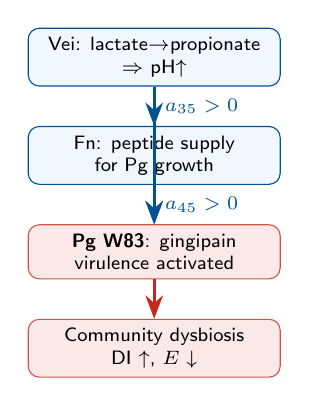
\begin{tikzpicture}[>=Stealth,node distance=0.5cm,font=\sffamily\scriptsize]
        \node[draw=ikm,rounded corners,fill=ikmxlight,minimum width=3.2cm,align=center]
          (vei) {Vei: lactate$\to$propionate\\$\Rightarrow$ pH$\uparrow$};
        \node[draw=ikm,rounded corners,fill=ikmxlight,minimum width=3.2cm,align=center,
              below=of vei] (fn)
          {Fn: peptide supply\\for Pg growth};
        \node[draw=red2!80,rounded corners,fill=red2!10,minimum width=3.2cm,align=center,
              below=of fn] (pg)
          {\textbf{Pg W83}: gingipain\\virulence activated};
        \node[draw=red2!80,rounded corners,fill=red2!10,minimum width=3.2cm,align=center,
              below=of pg] (dis)
          {Community dysbiosis\\DI $\uparrow$, $E\downarrow$};
        \draw[->,very thick,ikm]  (vei) -- node[right]{\scriptsize$a_{35}>0$} (fn);
        \draw[->,very thick,ikm]  (vei) -- (pg);
        \draw[->,very thick,ikm]  (fn)  -- node[right]{\scriptsize$a_{45}>0$} (pg);
        \draw[->,very thick,red2] (pg)  -- (dis);
      \end{tikzpicture}
      \vspace{3pt}
      {\scriptsize MAP values: $a_{35}^{\mathrm{DH}}=$ estimated;\;
       $a_{45}^{\mathrm{DH}}=5.63$ (strong Fn--Pg coupling)}
  \end{columns}
\end{frame}

% ── C: Additional Results ─────────────────────────────────────────────────────

\begin{frame}[plain]{C1. Corner Plot: DH Baseline Key Parameters}
  \vspace{-2pt}
  \centering
  
\includegraphics[height=0.86\textheight,keepaspectratio]{Fig19_corner_plot_dh_key_params.png}
  \par\vspace{2pt}
  {\scriptsize DH baseline posterior (Phase 2).
   Selected key parameters.
   Diagonal: marginal posteriors.
   Off-diagonal: joint distributions.
   Star: MAP.}
\end{frame}

\begin{frame}[plain]{C2. Basin Sensitivity: Multi-Attractor Landscape}
  \vspace{-2pt}
  \centering
  
\includegraphics[height=0.80\textheight,keepaspectratio]{Fig16_basin_sensitivity.png}
  \par\vspace{2pt}
  {\color{midgray}\rule{0.88\textwidth}{0.3pt}}\par
  {\scriptsize
   CS: 49/51 perturbed posterior samples jump to DI$\approx$0.85 attractor.
   DH real posterior: bimodal DI $[0.16,\,0.87]$.
   Basin filter threshold $= 0.25$.}
\end{frame}

\begin{frame}[plain]{C3. NUTS vs.\ HMC vs.\ RW-TMCMC Comparison}
  \vspace{-2pt}
  \centering
  
\includegraphics[height=0.82\textheight,keepaspectratio]{Fig21_nuts_comparison.png}
  \par\vspace{2pt}
  {\color{midgray}\rule{0.88\textwidth}{0.3pt}}\par
  {\scriptsize
   GPU RW-TMCMC: 500p$\times$9 stages $=$ 146.7\,s.
   NUTS acceptance: $1.75\times$ vs.\ RW (avg 0.93 vs.\ 0.53).
   NUTS/HMC not GPU-practical (warp divergence).}
\end{frame}

\begin{frame}[plain]{C4. DeepONet Surrogate: $\sim$100$\times$ Additional Speedup}
  \vspace{-2pt}
  \centering
  
\includegraphics[height=0.82\textheight,keepaspectratio]{Fig22_deeponet_posterior_comparison.png}
  \par\vspace{2pt}
  {\color{midgray}\rule{0.88\textwidth}{0.3pt}}\par
  {\scriptsize
   DeepONet-TMCMC: 12--18\,s vs.\ $\sim$1800\,s (GPU ODE).
   DH posterior overlap: 17/20 params $>$ 0.95, mean $=$ 0.903.}
\end{frame}

\begin{frame}[plain]{C5. $n$-Sensitivity and Percolation Justification ($n=2$)}
  \vspace{-2pt}
  \centering
  
\includegraphics[height=0.82\textheight,keepaspectratio]{Fig24_n_sensitivity.png}
  \par\vspace{2pt}
  {\color{midgray}\rule{0.88\textwidth}{0.3pt}}\par
  {\scriptsize
   Stiffness ordering CS$\geq$CH$>$DH$\gg$DS invariant $\forall n\in[1,3]$;
   BF$>10^6$ $\forall n$ (decisive).
   CS/DS ratio: $6\times$ ($n=1$) $\to$ $29\times$ ($n=2$) $\to$ $75\times$ ($n=3$).
   $n=2$ justified by 3D rigidity percolation $f\approx2.0$ (Sahimi 1994).}
\end{frame}

\begin{frame}[plain]{C6. Viscoelastic Extension (SLS Model)}
  \vspace{-2pt}
  \centering
  
\includegraphics[height=0.82\textheight,keepaspectratio]{Fig25_stress_relaxation.png}
  \par\vspace{2pt}
  {\color{midgray}\rule{0.88\textwidth}{0.3pt}}\par
  {\scriptsize
   Standard Linear Solid (Zener) model: $E_\infty(\mathrm{DI}) + E_1\,e^{-t/\tau}$.
   CS: $\tau=56.5$\,s, DS: $\tau=3.2$\,s.
   Quasi-static valid for $t\to\infty$: deviation $<0.3\%$.
   VE matters only for $t<\tau$ (3--57\,s transient loading).}
\end{frame}

\begin{frame}[t]{C7. Three-Model Comparison and Bayes Factor}
  \small\vspace{-2pt}
  \begin{columns}[T]
    \column{0.55\textwidth}
      \centering
      
\includegraphics[width=\linewidth,height=0.58\textheight,keepaspectratio]{Fig17_3model_comparison.png}
      {\scriptsize 3-model comparison: DI, $\phi_{\mathrm{Pg}}$, $\epsilon$ (EPS) index.
       CS/CH condition — all 4 conditions shown in full paper.}
    \column{0.43\textwidth}
      \begin{block}{Bayes factor summary (CS--DH pair)}
        \renewcommand{\arraystretch}{1.1}
        \begin{tabular}{@{}lrr@{}}
          \toprule
          \textbf{Model} & $\ln\hat Z$ & \textbf{BF vs.\ DI}\\
          \midrule
          DI (ours)   & best & 1\\
          Composite   & & $\times 2965$\\
          EPS-only    & & $\times5\times10^6$\\
          $\phi_{\mathrm{Pg}}$ & & fails ($<0.03$)\\
          \bottomrule
        \end{tabular}
      \end{block}
      \vspace{5pt}
      \begin{alertblock}{DI model is optimal}
        \begin{itemize}\setlength{\itemsep}{1pt}
          \item Dysbiotic = So-dominated (not Pg)
          \item $\phi_{\mathrm{Pg}}<0.03$ in all conditions:\\ cannot distinguish
          \item DI (Shannon entropy) captures\\ community-level disorder
        \end{itemize}
      \end{alertblock}
  \end{columns}
\end{frame}

\begin{frame}[t]{C8. Full Metrics Table and Convergence Diagnostics}
  \small\vspace{-2pt}
  \begin{columns}[T]
    \column{0.56\textwidth}
      \centering
      \renewcommand{\arraystretch}{1.1}
      \begin{tabular}{@{}l rrr rrr@{}}
        \toprule
        & \multicolumn{3}{c}{\textbf{Phase 1}} & \multicolumn{3}{c}{\textbf{Phase 2}}\\
        \cmidrule(lr){2-4}\cmidrule(lr){5-7}
        \textbf{Cond.} & RMSE & MAE & $M$ & RMSE & MAE & $\ln\hat Z$\\
        \midrule
        CS & 0.119 & 0.077 & 5 & 0.119 & 0.075 & $-3.3$\\
        CH & 0.071 & 0.053 & 6 & 0.104 & 0.088 & $-8.5$\\
        DS & \hl{0.020} & \hl{0.025} & 4 & \hl{0.033} & \hl{0.024} & $\mathbf{-2.8}$\\
        DH & 0.067 & 0.045 & 7 & 0.087 & 0.060 & $-11.9$\\
        \bottomrule
      \end{tabular}
      {\scriptsize $M$: number of TMCMC stages (Phase 1)}
      \vspace{5pt}

      \textbf{Phase consistency (Pearson $r$):}
      \begin{tabular}{@{}lcccc@{}}
        \toprule & CS & CH & DS & DH\\\midrule
        $r$ & 0.87 & 0.68 & 0.42 & 0.62\\
        \bottomrule
      \end{tabular}
    \column{0.42\textwidth}
      \begin{block}{Convergence diagnostics}
        \begin{itemize}\setlength{\itemsep}{2pt}
          \item $\bar\alpha=7$--13\% (all conditions)
          \item ESS $=N_p$ at final stage
          \item Gelman--Rubin $\hat R<1.1$ (all 15 params, 2 chains)
          \item DH posterior overlap (chain A vs.\ B): 17/20 params $>0.95$
        \end{itemize}
      \end{block}
      \vspace{5pt}
      \begin{block}{Model parsimony}
        Compression ratio $r_i=\sigma_{\mathrm{post},i}/\Delta_{\mathrm{prior}}$:
        \begin{itemize}\setlength{\itemsep}{1pt}
          \item Max across all: $r_i<0.43$
          \item DS mean: $r=0.07$ (tightest)
          \item Pg commensal: $r_i\leq0.10$
        \end{itemize}
        All params data-informed: no prior domination.
      \end{block}
  \end{columns}
\end{frame}

% ── Bibliography (hidden) ─────────────────────────────────────────────────────
\begin{frame}[allowframebreaks]{References}
  \tiny
  \bibliographystyle{unsrtnat}
  \bibliography{../data_5species/docs/references_ikm}
\end{frame}

% =============================================================================
\end{document}
